\chapter{Introduction}
\label{cha:intro}

%Heating, Ventilation and Air-Conditioning (HVAC) dominates the building electricity demand. 
Buildings are the largest consumer of energy worldwide, accounting for around 40\% of the world's energy supply \citep{macDonald2004commercial}. Within a building, heating, ventilation and air-conditioning (HVAC) systems consume the most energy, leading to trillion dollars of electrical expenditure worldwide each year. 

%TODO: Refer to Johnson Control and talk about optimisation in HVAC control. citep them all. (Johnson control etc those in ur patent)

Recent statistics show that, in the United States, offices and universities expend about 31\% of the total electricity consumption in the commercial building sector.\footnote{Commercial buildings consist of buildings used for education, food sales, food service, healthcare, lodging, mall \& mercantile, office, public assembly, public order and safety, religious worship, service, warehouse and storage and others.} This is equivalent to 387 billion kWh of electricity per annum \citep{eia2012cbecs}\footnote{See Table E5 at https://www.eia.gov/consumption/commercial/data/2012/c\&e/pdf/e5.pdf}. Amongst that, nearly 40\% of the consumption is used for space heating, cooling and ventilation. 

Similar consumption patterns are shown in Australia. % whilst its energy consumption is relatively lower than the United States. 
Both office and university buildings utilise approximately 12 billion kWh of electricity per annum. HVAC is responsible for a substantial portion of the energy used - approximately 46\% of the total building electricity consumption \citep{pitt2012baseline}. Figure \ref{intro:electricity_end_use_split} illustrates a breakdown of the electricity consumption in commercial offices and universities in the United States and Australia. %The statistics epitomize the end-use split of electricity consumption in most commercial offices and universities worldwide.
While these graphs reflect only statistics from 
\begin{figure}[hb]
\centering
%\begin{tabular}{c}
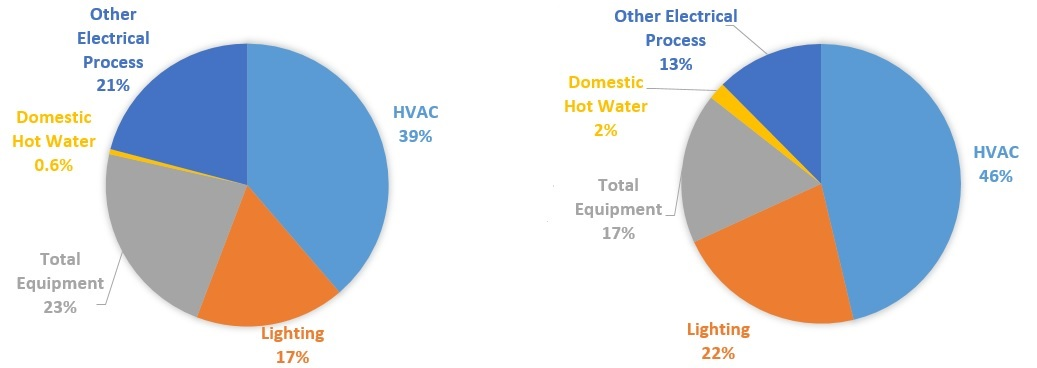
\includegraphics[width=5in,keepaspectratio]{figs/intro_end_use_split.jpg}
%\end{tabular}
\caption{Electricity consumptions of commercial offices and universities by end use in the United States (left) \& Australia (right).}
\label{intro:electricity_end_use_split}
\end{figure}
\noindent two countries, they epitomize the end-use split of electricity consumption in most commercial offices and universities worldwide.

With rising energy costs and increasingly stringent regulatory environments, improving the energy efficiency of HVAC operations in buildings has become an important issue. From a short-term economic point-of-view, with over 100 billion dollars in annual electricity expenditures even a small percentage improvement in the operation of HVAC systems can lead to significant savings. From a long-term point-of-view, the need of fostering a smart and sustainable built environment calls for the development of innovative HVAC control strategies in these buildings. 

%--------------------------------------------------------------------------------------

\section{Problem Addressed}
\label{sec:problemstatement}
%I believe A is better than B.
 
There are substantial opportunities to reduce the HVAC energy consumption in commercial offices and universities, given their significant energy consumption. %through optimisation. 
%Occupants’ HVAC usage is largely dependent on their activities.
%Appropriate scheduling of the occupants’ activities in commercial/educational buildings helps to proactively control HVAC operations.

In conventional building operations, HVAC systems run according to a pre-defined occupancy schedule. They maintain a minimum air flow rate to ensure prescribed indoor air quality standards, and keep the zone temperature within a pre-defined comfort range using real-time temperature measurements in a {\em reactive} manner. One weakness of this control logic is that it ignores occupancy dynamics: it treats unoccupied zones of the building in the same way as occupied ones, which results in substantial energy waste.

Recent studies have shown that energy consumption can be significantly improved by adopting more complex control strategies that exploit measured or predicted occupancy information \citep{agarwal2010occupancy, erickson2010occupancy, erickson2009energy, goyal2013energy, goyal2013occupancy, west2014trial}. For instance, model {\em predictive} control strategies determine supply air flow rate and temperature over longer time horizons in such a way as to optimise energy consumption, whilst remaining within air flow and temperature bounds that reflect the predicted occupancy of various building zones \citep{goyal2013occupancy}. These strategies are naturally capable of pre-cooling zones if this reduces consumption or if it is necessary to meet the comfort bounds. %However, these approaches do not perform occupancy scheduling, and ignore the fact that some schedules may lead to more energy savings. 

Another body of recent research has investigated the {\em proactive} control of {\em occupancy} in order to minimise HVAC consumption \citep{chai2014minimizing,klein2012coordinating,kwak2013tesla,majumdar2012energy,pan2012thermal}. Many office and university buildings offer some scope for occupancy control via their room booking and scheduling systems. For instance meetings, lectures, exams, use of special purpose rooms, and other short-term activities can be scheduled to occur at times and in rooms that are beneficial from an energy standpoint.
Unfortunately, existing occupancy scheduling approaches assume conventional HVAC control strategies \citep{kwak2013tesla}. Moreover, since working from first principles using models of the HVAC and the building is computationally expensive, they typically adopt suboptimal scheduling strategies guided by proxies for the optimisation criterion. One such proxy is the minimisation of the number of rooms used and of the time gap between successive meetings; it is used to guide the search towards solutions that take advantage of thermal inertia and schedule meetings to take place back-to-back in as few rooms as possible \citep{pan2012thermal,majumdar2012energy}.

In this thesis, we go an important step beyond existing work: we look at the potential for integrating building operations with room booking and occupancy scheduling, and combine the benefits of both research trends above. 
%Specifically, energy consumption in commercial offices and educational buildings is impacted by group activities such as meetings, workshops, classes and exams, and can be reduced by scheduling these activities to take place at times and locations that are favorable from an energy standpoint. 
More specifically, we explore a new way of reducing HVAC consumption in commercial buildings, by jointly optimising the occupancy scheduling decisions and the building's occupancy-based HVAC control. %, by allowing the occupancy scheduling decisions to rely on an explicit model of the building's occupancy-based HVAC control. 

As mentioned before, existing work considers either one or the other subproblem: either scheduling occupancy given conventional control policies, or HVAC control using a given occupancy schedule. 
From a computational standpoint, the joint problem is much more challenging than either, as HVAC models are traditionally non-linear and non-convex, and scheduling models additionally introduce discrete variables capturing the time slot and location at which each meeting is scheduled. This problem is regarded as a non-linear hybrid discrete-continuous problem, which is challenging to solve and optimise. A core aspect of this research will thus be to design models that are amenable to optimisation, while being sufficiently accurate. 

The key research question we tackle in this context poses a substantial challenge but can be expressed concisely:
\begin{quotation}
		\emph{Can we design optimisation methods that integrate occupancy scheduling with HVAC control, in such a way that the HVAC consumption is reduced, while the occupancy thermal comfort and scheduling requirements are addressed?}
\end{quotation}

In answering this question, we will provide a holistic approach that improves the energy efficiency of HVAC operations in buildings over state-of-the-art mechanisms. This will allow the HVAC systems to operate more efficiently and at lower cost. Building occupants will benefit through effective controls that assure their thermal comfort, while reducing their carbon footprint.

We identify four unique research challenges that should be simultaneously addressed in order to achieve our goal, which form the motivations for the work in this thesis:
\begin{enumerate}
  \item The integrated model should be computationally \emph{efficient} and achieve optimal energy reduction by fully exploiting the capability to coordinate HVAC control and occupancy scheduling. 
	\item Given sets of occupancy schedules with different constrainedness and sets of buildings with varying thermal response, the model should be sufficiently \emph{scalable} to provide instantaneous and near-optimal solutions to control and scheduling problems of realistic size.
	\item The model should be able to handle impromptu scheduling requests and respond in an \emph{online} manner.
	\item The model should enable \emph{flexible} and \emph{robust} control and scheduling, by considering the dynamics of external weather and occupants' thermal comfort preferences. 
\end{enumerate}

When combined, these parts deliver a novel mechanism that is efficient, scalable, flexible and robust for \emph{energy-aware occupancy scheduling} in commercial buildings.


%--------------------------------------------------------------------------------------
\section{Contributions}
\label{sec:contributions}
%The main challenge is that the HVAC system is rather complex and an optimisation model should model them at the proper level of abstraction to obtain optimisation models that can be solved in reasonable time. 

\subsection{Integrating HVAC Control with Occupancy Scheduling}

The first key contribution of this thesis is an integrated model that solve a \emph{joint} HVAC control and occupancy scheduling problem \citep{lim2015hvac}. Existing approaches typically solve these subproblems in isolation. A na\"{\i}ve combination would be to schedule occupancy in a first phase using existing methods, and then control HVAC based on this occupancy schedule. In contrast, we model and solve the {\em joint} HVAC control and occupancy scheduling problem. This results in an integrated approach whose benefits exceed the na\"{\i}ve superposition of both of its parts, as the scheduling fully exploits the capabilities of the underlying occupancy-based HVAC control across available times and locations.

In more detail, the joint problem we consider is that of deciding the respective times and locations (rooms) of a set of meetings or similar
activities, as well as the HVAC supply air temperature and air flow rate for each zone and time, in such a way as to optimise the overall
HVAC consumption over a long time horizon. The schedule complies with the HVAC and building dynamics models, and with comfort and air flow
rate bounds that depend on the scheduled zone occupancy. It also satisfies typical meeting scheduling constraints, including constraints on meetings times, on meeting locations (e.g. room capacity, equipment availability), and on participant attendance conflicts. 

\begin{figure}[ht]
\centering
\begin{tabular}{c}
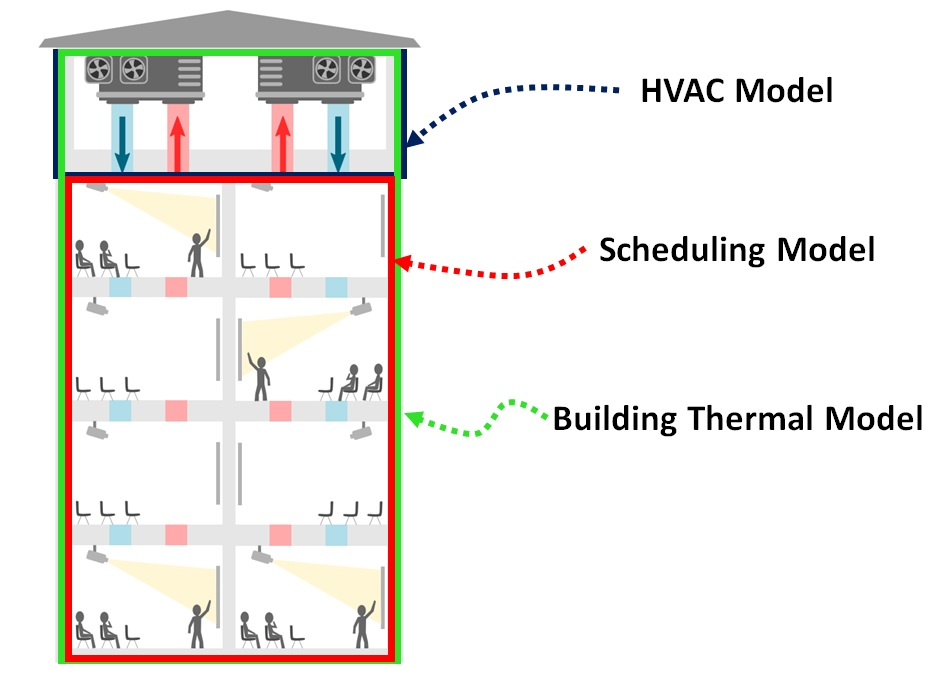
\includegraphics[width=5in,keepaspectratio]{figs/intro_three_models.jpg}
\end{tabular}
\caption{Integrated HVAC control and occupancy scheduling.}
\label{intro:three_models}
\end{figure}

Figure \ref{intro:three_models} illustrates the integration of HVAC control and occupancy scheduling in a building. To achieve this, the joint model we develop consists of three core-components: 
\begin{enumerate}
		\item A HVAC control model that simulates the physical HVAC system and allows controlling its operations, %a HVAC model that simulates the physical system of HVAC operations in buildings,
		\item a building thermal model that simulates the thermal dynamics based on internal and external heat gains, and
		\item an occupancy scheduling model that incorporates the occupancy activities, preferences and requirements.
	\end{enumerate}

Following Goyal et al. \citep{goyal2012method,goyal2013occupancy}, we focus on variable-air-volume (VAV) based HVAC systems, which serve over 30\% of the commercial building floor space in the United States \citep{eia2012cbecs}. The VAV-based HVAC systems allow us to model zone-based HVAC control, which is a crucial component for occupancy-based HVAC control. This model incorporates fan, air-conditioning and heating operations of each zone in the building, and estimates the energy consumption as a function of the HVAC control inputs (i.e. the conditioned air temperature, outdoor temperature, supply air temperature and flow rate). 

We adopt a lumped resistance-capacitance (RC)-network to model the building thermal dynamics. This model incorporates building thermal resistance, thermal capacitance, solar gain, internal heat gain and enthalpy into the estimation of zone temperature fluctuation. As buildings with different build-up (such as walls' materials, windows' facing etc.) possess different indoor climate conditions, we consider buildings with different thermal resistances and thermal capacitance. This allows us to demonstrate the energy-efficiency of different building types, and showcase the importance of picking the right rooms and times for energy savings.

Our scheduling model takes a list of meeting requests consisting of meeting time windows, duration of the meeting, list of attendees, and optionally a preferred room. We consider schedules with smaller size and constrainedness in the initial stage of our work, demonstrating the benefit of our model over existing approaches. We then introduce schedules with higher complexity and constrainedness to showcase the scalability of the model.

When combined, these three core components form an integrated model that determines the times and locations of a set of occupant activities, and a set of HVAC control inputs (i.e. the supply air temperature and air flow rate) for each zone, in such a way as to minimise HVAC consumption.

Our initial model consists of a mixed-integer non-linear programming (MINLP) model. What makes this especially challenging is the presence of bilinear terms in the HVAC control, which involves non-linear non-convex constraints. To address the challenges caused by the presence of non-linear HVAC control constraints, we relax them in a principled way using McCormick's relaxation to obtain a mixed-integer linear (MILP) model guaranteed to provide a lower bound on the objective function. Given the highly-constrained nature of meeting scheduling with HVAC control, solving the integrated problem as a MILP seems to be a reasonable choice. MILP easily manages the interaction between meeting scheduling and the impact it has on HVAC energy consumption.

%We then introduce the concept of outdoor air economy cycle into our integrated model. Economy cycle is a strategy of using 100\%of ourside air to provide ``free cooling'' when conditions permit.  %The presence of discrete variables in our HVAC model facilitates the introduction of a standby mode for operating out of business hours. 
As a further refinement, we then introduce a HVAC standby mode for operating out of business hours in our integrated model. In conventional operations, the HVAC is turned off outside of business hours (typically 6pm-6am) and restarts early in the morning to ensure that building temperature is comfortable by start of business. With our standby mode, the HVAC can decide to re-activate at night if this results in reduced consumption. Perhaps surprisingly, we show that in certain circumstances, anticipating an early morning meeting by activating the HVAC at night to cool the supply air whilst the outside temperature is still low, can reduce consumption over waiting for the pre-defined HVAC turn on time. This feature also greatly improves the \textsl{feasibility} of the solution by activating the HVAC over night to achieve targeted occupied room temperature on the next day.
%To ensure the existence of a feasible control (for adequately sized HVACs) and improve on current occupancy-based HVAC control   practices, we introduce a standby mode enabling the HVAC to re-activate at night if this is necessary to meet the temperature bounds of an early morning meeting or results in reduced consumption. 

Our results show that the integrated model achieves substantial reduction in energy consumption compared to the state of the art approaches using heuristic scheduling solutions and to more na\"{\i}ve integrations of meeting scheduling and occupancy-based HVAC
control. The MILP model developed is efficient enough for occupancy-based HVAC control, and can be used in a range of applications. Once built, such a schedule can be used in any building equipped with an occupancy-based HVAC controller by simply complementing the occupancy forecast \citep{mamidi2012adaptive} with the occupancy information captured in the schedule. Our approach can even be used with a conventional HVAC control system by constraining the bounds on supply air flow rate/temperature and the temperature setpoints to be those found in the optimal solution to the joint problem. 

\subsection{Scaling to Large Problems}

% say meetings arrival etc.
% say results show destroy room based in superior
%Large neighourhood search (LNS) model, which is approximate, and yet, precise enough to identify better quality solution within short time limit.
% Furthermore, we claim that our mechanism is \textsl{scalable} to solve control and scheduling problems with different size of complexity and constrainedness. Consequently, we will design and develop models that are capable of solving large-scale problems.

Statistics show that meeting frequency in commercial buildings is significant and continues to grow \citep{romano2001meeting,kim2014learning}. In the United States alone, fortune 500 companies are estimated to hold 11 million formal meetings daily and 3 billion meetings annually \citep{romano2001meeting}. Amongst that, 83\% of the meetings last up to 2 hours \citep{kim2014learning}. From another survey collected from the University of Southern California \citep{kwak2013tesla}, there are daily 300 unique meetings per regular day across 35 group study rooms in their university's library.

This motivates our next step where we expand our integrated model to solve large-scale problems. Our second contribution in this thesis is a Large Neighbourhood Search (LNS) approach that is capable of handling hundreds of incoming meeting requests across a large number of offices/rooms \citep{lim2015large}. The scale of control and scheduling problems grow exponentially with the number of meetings and locations. The exact method using MILP is typically too expensive for such large scale instances. Hence, to tame the problem complexity further and scale to large problems, we combine the MILP model with LNS. 

LNS is a technique for finding good or near-optimal solutions via iterative optimisation through multiple destroy and repair steps in smaller neighbourhoods. LNS is used in the destroy step to remove all meetings in a small number of randomly selected zones. MILP is used in the repair step to solve the resulting subproblem and repair the schedule to near-optimality within a limited runtime. %to form a subproblem that is capable of repairing schedule to near-optimal within a limited runtime. 
This hybrid model allows us to easily navigate through the solution space and escape local minima.

One crucial criteria of this approach is the need of identifying optimal LNS parameters that govern the behavior of the LNS heuristics. There are two key parameters to tune: (a) the number of rooms to destroy, and (b) the MIP runtime limit for the repair step. One important decision when implementing the destroy step is determining the amount of destruction. If too little is destroyed the effect of a large neighbourhood is lost and if too much is destroyed then the approach turns into repeated re-optimisation. Another important decision is whether the repair step should be optimal or not. An optimal repair will be slower than a heuristic, but may potentially lead to high quality solutions in a few iterations. 

There are numerous values that these parameters can take on. As a result, some parameter tuning will be essential in achieving good performance overall. We use the sequential model-based algorithm configuration (SMAC) methodology \citep{hutter2011sequential} on an independent set of problems to optimise the parameters of the number of rooms to destroy and the MILP run time. Specifically, we generate problem instances with different degrees of constrainedness and train the parameters to achieve the best quality for all input scenarios.

What we find in our experiments is that this approach is reasonably responsive and fast in providing near-optimal solutions. Given benchmark sets of different complexity and constrainedness, the model outperforms the MILP model in terms of (a) solution optimality given a time limit, and (b) solution feasibility of the HVAC control and occupancy scheduling.


\subsection{Handling Online Requests}
%to cope with online meeting requests while regulating optimal HVAC control. 

Our third contribution is an \emph{online} approach that models and solves the joint HVAC control and occupancy scheduling problem \citep{lim2016online}. The previous two approaches are offline methods: they assume that all activities to schedule and other parameters such as the weather forecast and the solar gain are known in advance. Although both settings generate energy-efficient schedules, they nevertheless limit the practicability of the models in the real world. A recent survey shows that 56\% of meeting requests were made within 1 day before the actual meeting day \citep{kwak2013tesla}. Thus, the ability to handle impromptu requests is crucial. Moreover, the ability to update HVAC controls following a change in forecast is also essential.

Our online algorithm greedily optimises and commits to the times and locations for the latest requests, leaving the rest of the current meeting schedule fixed but revising the entire future HVAC control strategy. This ensures that whilst participants are instantly notified of the scheduled time and location for their requested activity, the HVAC control is constantly re-optimised and adjusted to the full schedule and weather updates. 

As in the offline case, we formulate the online model using mixed-integer programming (MIP), and combine MIP with large neighbourhood search (LNS) so as to scale to problem with large number of online requests and building zones. Given the relatively smaller number of meetings in online scheduling compared to offline scheduling (while the search space remains large in terms of the number of building zones), this hybrid model is highly efficient in finding near-optimal solutions. Our experiments demonstrate that the quality of the online solution is, on average, within 1\% of that of the solution returned by the clairvoyant offline HVAC-aware algorithm \citep{lim2015large}.

\subsection{Enabling Adaptive Temperature Control}

The final contribution of this thesis explores adaptive temperature control in our joint HVAC control and scheduling model \citep{lim2016online}. Existing approaches typically assume fixed comfort bounds on the occupied zone temperature. In the fixed comfort bounds model, when a zone is occupied, the zone temperature must lie within standard cooling and heating setpoints (e.g. 21$^\circ$C-23$^\circ$C). We introduce the notion of \textsl{thermal comfort flexibility} by departing from these fixed comfort bounds. Instead of keeping the room temperature within standard setpoints, the occupants are encouraged to conserve energy by accepting some temperature deviation from the default setpoints. %They are allowed to indicate their level of tolerance to temperature fluctuation.
To achieve this, we formulate adaptive temperature models that leverage occupants' thermal comfort flexibility and outdoor temperature, and use them in a principled way to decide occupants' schedules and optimise HVAC control. 

Specifically, we explore two adaptive temperature control schemes: (a) the maximum temperature deviation aware approach (MTDA), and (b) the outdoor temperature aware approach (OATA). The first scheme limits the maximum temperature deviation allowed at any time throughout the activity period, whilst the second scheme considers the outdoor temperature. We first define a deterministic model that calculates a \textsl{cumulative temperature violation} threshold based on the selected scheme. This threshold bounds the total temperature deviation throughout the activity period, enabling adaptive temperature control whilst assuring that the thermal comfort is kept within the occupants' tolerance level. 
Whilst the deterministic model is simplistic and effective, it is hard to cope with the uncertainties on the thermal flexibility of every occupant in a meeting. To cope with these uncertainties, we resort to a robust optimisation approach. In particular, we adopt the ellipsoidal uncertainty sets approach, and provide a probabilistic guarantee to the thermal comfort satisfaction level indicated by the occupants. 
Our experiments show that, when occupants are reasonably flexible, the integration of adaptive temperature control generates higher energy savings than the fixed temperature control approach.
%These configurations are carefully chosen to be realistic enough to demonstrate the advantage of adaptive temperature control, whilst assure that the thermal comfort standard defined by the ASHRAE Standard \citet{ashrae2013thermal} is observed.  

As an additional advantage, adaptive temperature control reduces the constrainedness of our online scheduling and control problem. This can make the problem solvable when fixed temperature bounds cannot be met, which often occurs for instance when a late request needs to be scheduled in the immediate future in a room whose current temperature is far away from the comfort band. In our experiments, adaptive temperature control solves a large number of instances that are unsolvable under the fixed temperature control model.

%The final contribution of this thesis explores adaptive temperature control in our joint HVAC control and scheduling model \citep{lim2016online}. According to \cite{de1998developing}, the occupants' thermal sensations are influenced by outdoor climate conditions. They proposed an adaptive comfort temperature scheme, which shifts away from fixed indoor comfort bands towards wider temperature operating bands based on outdoor temperature. Recent work \citep{egan2010the} shows that even a narrow variation of comfort temperatures can achieve significant energy savings. 

%We introduce the concept of robust optimisation into the online model in chapter \ref{cha:online}. Unlike the online approach with fixed temperature bound, in this robust formulation, the comfort constraints are relaxed in a way that allows the thermal comfort conditions to be violated for a limited amount of time. We implement both adaptive temperature control methods with three flexible comfort levels  defined: low, medium and high settings. Each setting has different input configurations that reflect the occupants' level of thermal comfort flexibility. These configurations are carefully chosen to be realistic enough to demonstrate the advantage of adaptive temperature control, whilst assure that the thermal comfort standard defined by the ASHRAE Standard \citet{ashrae2013thermal} is observed. 

%\textcolor[rgb]{1,0,0}{Need rewrite clearer!!!  Inspired by these works, we introduce the notion of thermal comfort flexibility in our model by allowing occupants to indicate their level of tolerance to temperature fluctuation. We explore two different schemes. The first scheme sets the maximum temperature deviation allowed any time, whilst the second scheme uses outdoor temperature to derive a threshold limiting the temperature violation. Both schemes are formulated into low, medium and high flexibility level, which simplify the occupant's choices for different tolerance ranges. We then solve a robust optimisation model which provides a probabilistic guarantees to the temperature violation threshold. Our experiments show that, when occupants are reasonably flexible, the integration of adaptive temperature control generates higher energy savings than the fixed temperature control approach.}


\section{Potential Integration with Building Management Systems}

We have developed a working prototype for the mathematical models discussed in Section \ref{sec:contributions}. In this section, we explore the potential of integrating this prototype with building management systems (BMS). 

%While it is possible to reduce energy consumption by retrofitting buildings with more efficient HVAC systems, it is far more cost effective to improve their control algorithms. A building management system (BMS) predominantly operates on a pre-designed schedule that incorporates a nighttime setback strategy, which relaxes the comfort constraints during the night. Bloomfield and Fisk \citep{bloomfield1977optimisation} show that such a strategy leads to significant energy savings. Building management systems, however, could be far more dynamic by adopting strategies that consider occupancy information. Occupants impact the thermal behavior of buildings. For example, a BMS may relax the comfort constraints for those rooms in the building that are not planned on being used.
%While some buildings use occupancy sensor measurements to adjust lighting and in some cases adjust both lighting and ventilation, the question we address in this paper is whether proactive planning and room management via \textsl{meeting scheduling} can have an increased impact on energy savings.

This is motivated by the fact that today's BMS tend to look at the building subsystems such as HVAC control, lighting control, blind control, plug load control in isolation, not exploiting the complementary functions of the various subsystems to minimise energy consumption. BMSs also tend to be rigid, not exploiting the wealth of information on existing and future building occupancy and the forecast energy load of the building. A significant opportunity lies in integrating room and occupancy scheduling into the BMS. Research has been conducted to develop integrated and intelligent BMS systems in smart buildings \citep{honeywell2016hvac,biq2014moving,biq2014managing,lu2012integrated,smith2011energy,klee2011seven}, however none of these systems consider integrating occupancy scheduling with building operations. Indeed, the BMS at reservation times should be capable of determining which rooms are most adequate from an energy-efficiency standpoint given the expected room occupancy, the predicted temperature profile of the building's zones and the forecast outdoor weather. 

\begin{figure}[ht]
\centering
\begin{tabular}{c}
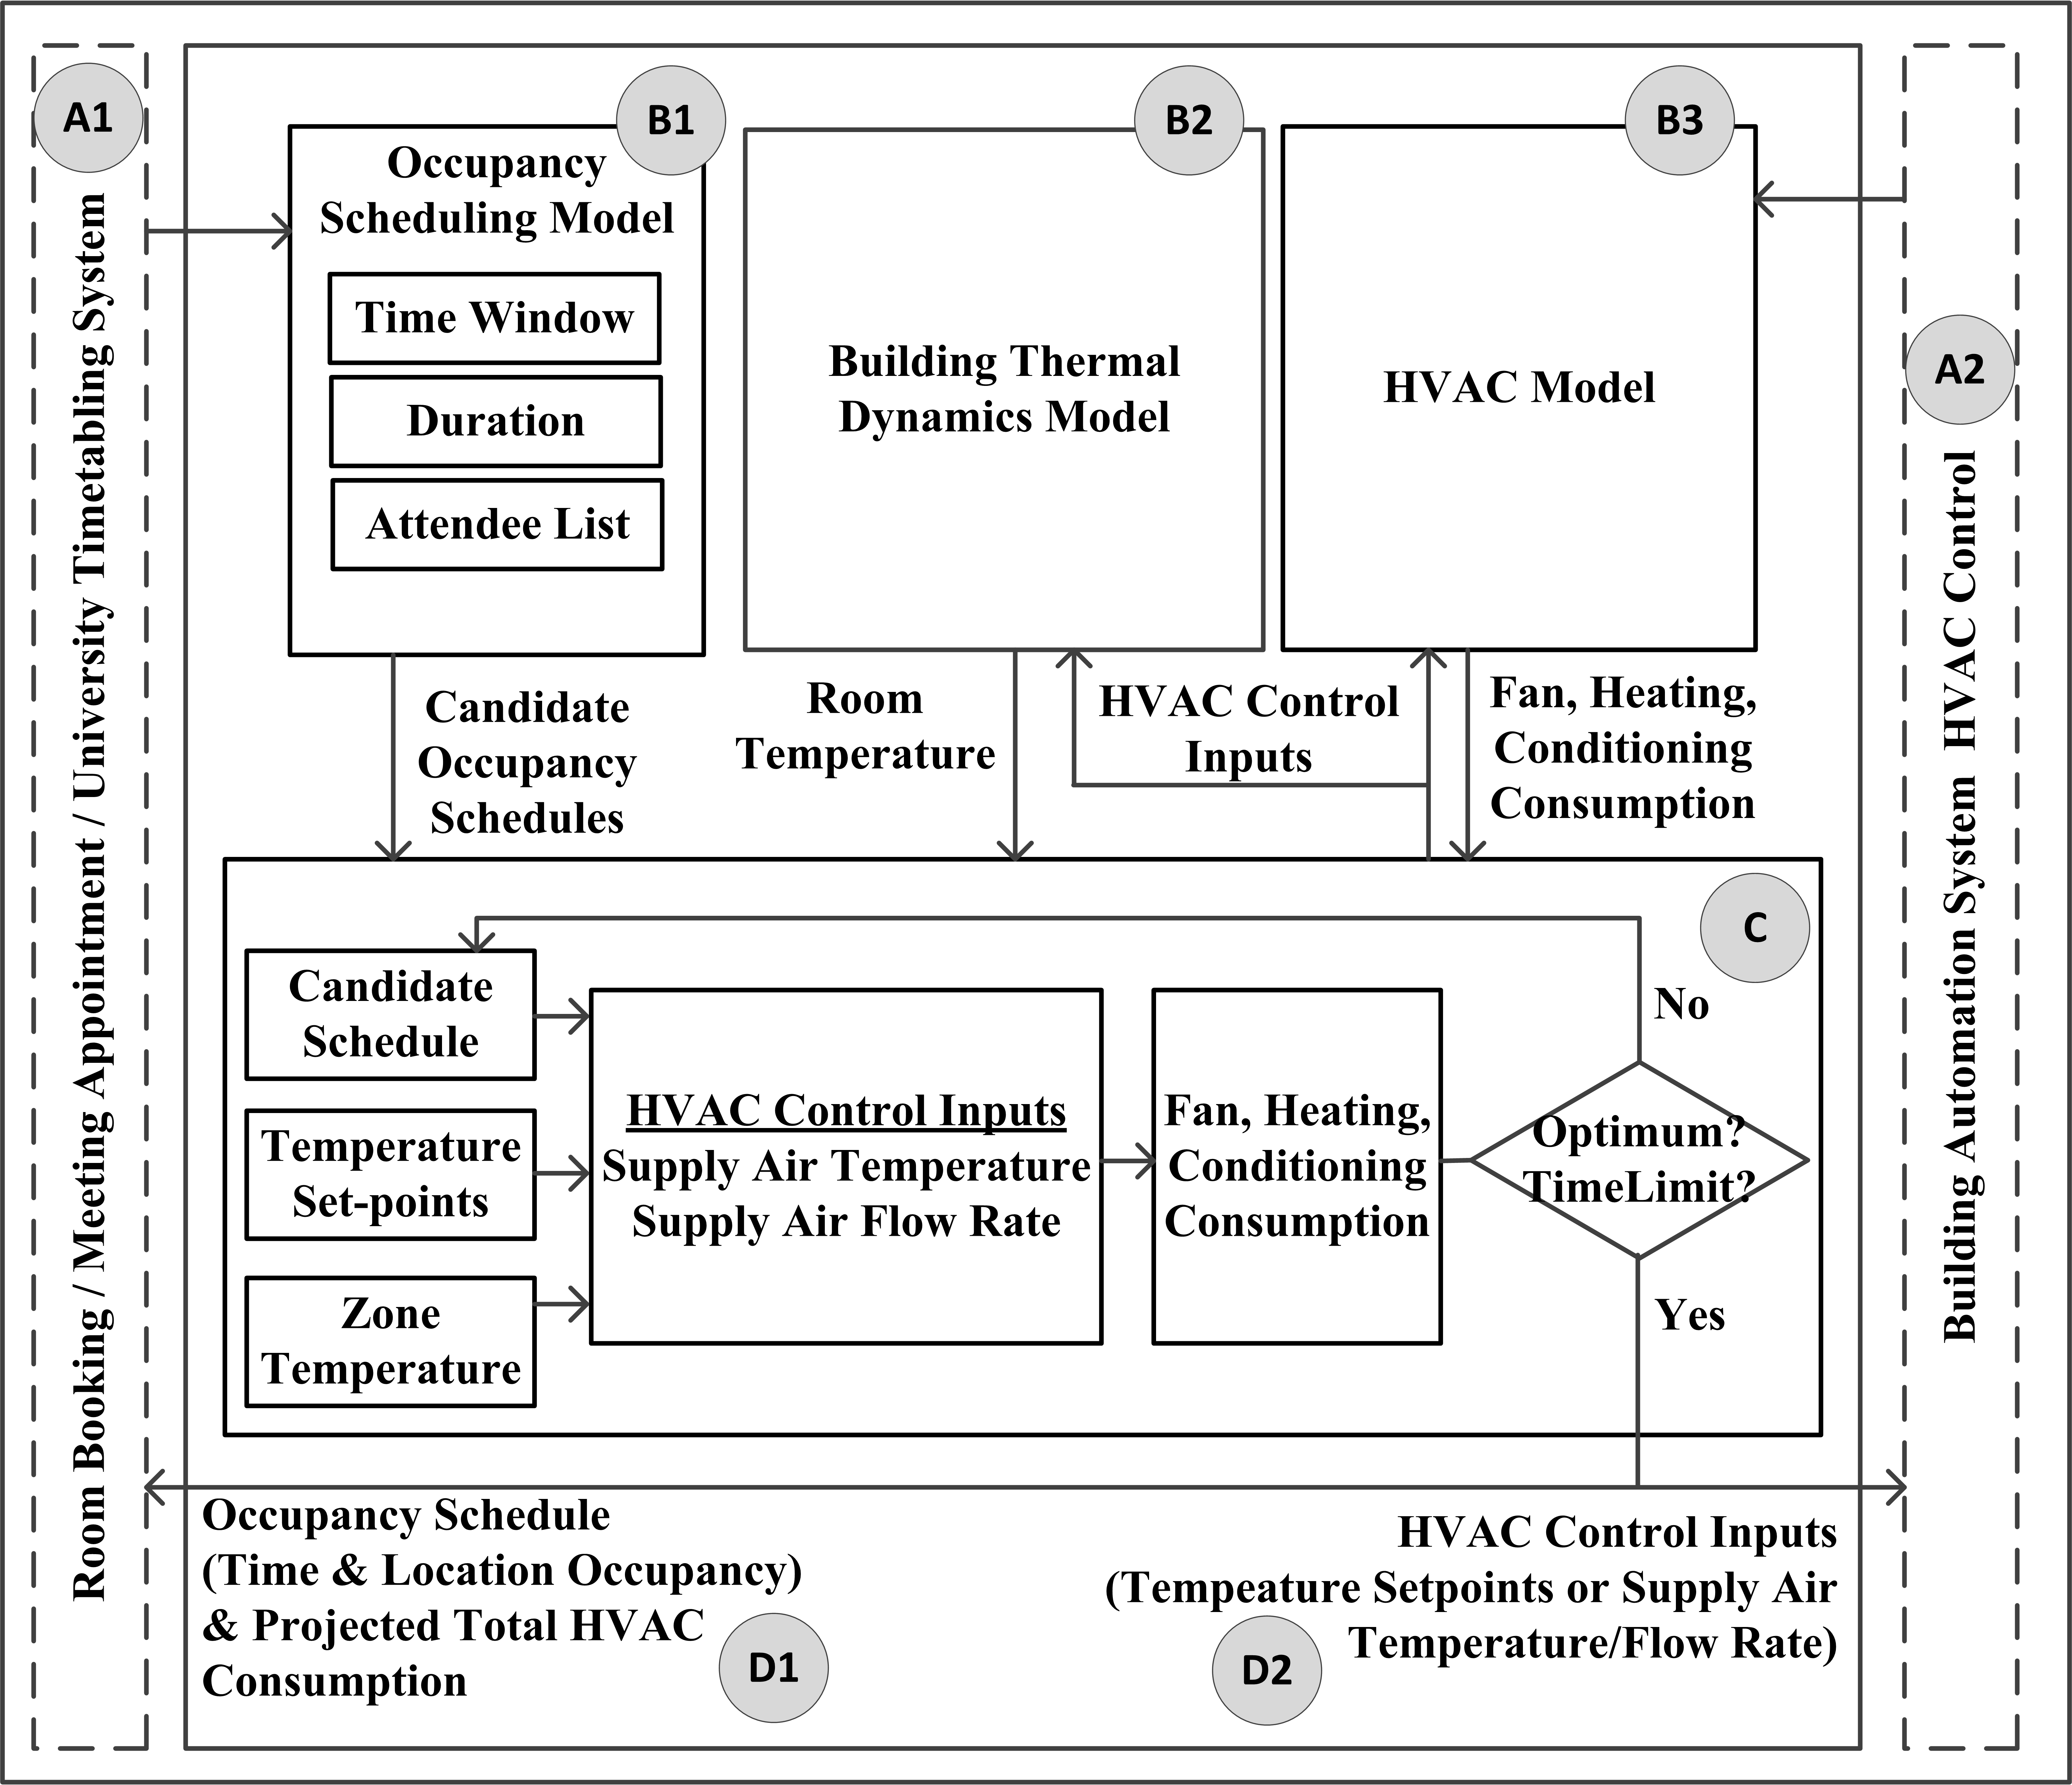
\includegraphics[width=4in,keepaspectratio]{figs/intro_eams.jpg}
\end{tabular}
\caption{Potential integration with building management system \& room booking systems}
\label{intro:eams}
\end{figure}

Figure \ref{intro:eams} illustrates how our software prototype can be integrated to the existing BMS system. This figure shows the input (label A), process (labels B \& C) and output (label D) of the integrated system. Our system receives the following as inputs:  
\begin{enumerate}
	\item a set of occupancy requests including time windows, duration, attendee list, and optionally their temperature flexibility, preferred locations and facilities required from the occupancy management system (A1). These system can be either a room booking system, a meeting appointment system or a timetabling system, and
	\item the buildings physical model, the components settings and the components limitations of the building's HVAC control from the Building Automation System (A2).
\end{enumerate}

These inputs allow us to calculate and configure appropriate constant values and constraints for the scheduling model (B1), the building thermal dynamic model (B2) and the HVAC model (B3). We then run our integrated model (C) to identify the optimal HVAC control and the best occupancy schedule that maximise energy efficiency while meeting occupant comfort needs. 

The outputs consist of
\begin{enumerate}
	\item An occupancy schedule (D1), given time and location of each request, and the projected total HVAC consumption,
	\item the HVAC control settings (D2), given the zones temperature setpoints, the zone's supply air flow rate and temperature over the scheduling horizon.
\end{enumerate}

The occupancy schedule and the projected total HVAC consumption can be delivered to the occupancy management system. This information allows building occupants to track their schedule and the overall HVAC consumption of the buildings. Currently, building occupants do not usually pay attention to \textsl{when} and \textsl{where} they use HVAC. Due to the lack of informed decision about energy savings, the selections of venue and time for an activity are often determined by their preferential choice. Now, with the energy consumption information provided, they are given an option to make an environmental friendly decision according to their schedule. 

The HVAC control scheme consists of the temperature setpoints, the supply air flow rate and temperature of each zone. This information can be selectively fed into the HVAC control system, depending on the granularity of control allowed. Currently, the temperature setpoint of each zone can be configured easily via the application programming interface of the BMS, thus this information can be used directly by constraining the comfort temperature of each zone based on our occupancy schedule. On the other hand, if the HVAC control allows a more fine-grained control, the  optimal supply air flow rate/temperature generated by our model can be used as setpoints.


\section{Summary}
\label{sec:intro_summary}

To summarise, the core research question we tackle is that how to design optimisation methods that integrate occupancy scheduling
with HVAC control, in a way that maximises energy savings whilst ensuring the comfort level necessary for occupants. We address this question in four parts that come together to form a complete solution: the formulation of a joint HVAC control and occupancy scheduling model, the development of a scalable joint model to solve large problems, the introduction of an online joint model that is capable of coping with impromptu meeting requests, and the integration of adaptive temperature control that further improves on the energy savings.

We contribute to knowledge in the area of energy-aware occupancy scheduling:
\begin{itemize}
	\item We formulate an integrated HVAC control and occupancy scheduling model using MILP, which produces efficient solutions compared to  existing approaches, and can be used in a range of applications,
	\item We develop a scalable model that combines MILP and LNS, and demonstrate that this hybrid model can effectively tackle large-scale HVAC control and meeting scheduling problems,
	\item We determine an online control and scheduling strategy based on a greedy algorithm that commits to the best schedule for the latest activity requests and notifies the occupants immediately, whilst simultaneously optimising the HVAC control parameters,
	\item We establish a robust optimisation model which enables adaptive temperature control and provides a probabilistic guarantee to the level of comfort tolerance indicated by the occupants.	
\end{itemize}

The key insight underlying this thesis is that integrating occupancy scheduling with HVAC control can lead to significant savings in energy consumption. By exploiting the synergy between HVAC control and occupancy scheduling, this approach achieves a much higher rate of energy savings than works that are based on (data-driven) black-box models of the HVAC control \citep{kwak2013tesla,chai2014minimizing} or that minimise energy consumption proxies (e.g. number of rooms used) \citep{majumdar2012energy,pan2012thermal}. Our work sets a baseline for the integration of HVAC control and occupancy scheduling in the space of energy aware scheduling in smart buildings.


\section{Thesis Outline}
\label{sec:outline}
%How many chapters you have? You may have Chapter~\ref{cha:background},
%Chapter~\ref{cha:design}, Chapter~\ref{cha:methodology},
%Chapter~\ref{cha:result}, and Chapter~\ref{cha:conc}.

This thesis is structured as follows:

Chapter 2 provides a non-technical introduction to occupancy-based HVAC control. It dedicates sections to discussing all related background: the concept of zone-based HVAC systems, building thermal model, occupancy-based control strategies, occupancy modeling and adaptive temperature control.
% the HVAC system and the building thermal model that we adopt. It also dedicates sections to discussing occupancy-based HVAC control and adaptive temperature control strategies that have been used in the HVAC domain.

Chapter 3 provides necessary background for the optimisation techniques that have been used to formulate our model. These include mixed integer programming (MIP), large neighbourhood search (LNS), online optimisation, and robust optimisation.

Chapter 4 introduces the joint HVAC control and occupancy scheduling problem, and develops an integrated model using MIP. We compare this model with the state-of-the-art occupancy-based HVAC control and heuristic-based occupancy aware scheduling, and show the corresponding experimental results.

Chapter 5 describes the LNS formulation, which integrates the MIP model with the LNS heuristics. We also discuss the automatic parameter tuning and our key observations.

Chapter 6 extends the integrated model to support online scheduling and control, and compares its effectiveness with the clairvoyant offline model.

Chapter 7 investigates the potential of adopting adaptive temperature control. We formalise the adaptive temperature control model based on robust optimisation method, experiment with different flexible setpoints control settings and demonstrate a further reduction of energy consumption compared to existing fixed temperature model.

Chapter 8 concludes our findings and combined approach, and discusses possibilities for future research.
